\documentclass [xcolor=svgnames, t] {beamer} 
\usepackage[utf8]{inputenc}
\usepackage{booktabs, comment} 
\usepackage[absolute, overlay]{textpos} 
\useoutertheme{infolines} 
\setbeamercolor{title in head/foot}{bg=internationalorange}
\setbeamercolor{author in head/foot}{bg=dodgerblue}
\usepackage{csquotes}
\usepackage[style=verbose-ibid,backend=bibtex]{biblatex}
\bibliography{bibfile}
\usepackage{fontawesome}
\usepackage{amsmath}



\usepackage{textpos}



\usetheme{Madrid}
\definecolor{myuniversity}{RGB}{0, 60, 113}
\definecolor{internationalorange}{RGB}{231, 93,  42}
 	\definecolor{dodgerblue}{RGB}{0, 119,202}
\usecolortheme[named=myuniversity]{structure}
\usepackage{tikz}



\title[Project Arctic Circle]{Project Arctic Circle}
\subtitle{Software Development}
\titlegraphic{\hfill
\includegraphics[height=1.5cm]{Fds.png}}
\author[A.SOW,C.FERNANDEZ, O.ESSBAI,S.DJOUAHRA]{{Fernandez Christelle, Sow Oumouratou Anna
,Es-Sbai Omar, Djouahra Sonia } \\
\faGithub\href{https://github.com/ChristelleFDZ/projectarcticcircletheorem/}{ Arctic Circle theorem} }

\institute[]{Masters MIND-Biostatistic, Montpellier University}



\date{April 25, 2021}


\addtobeamertemplate{navigation symbols}{}{%
    \usebeamerfont{footline}%
    \usebeamercolor[fg]{footline}%
    \hspace{1em}%
    \insertframenumber/\inserttotalframenumber
}

\begin{document}


\begin{frame}
 \titlepage   
\end{frame}

\begin{frame}{Introduction}
\begin{figure}[t]
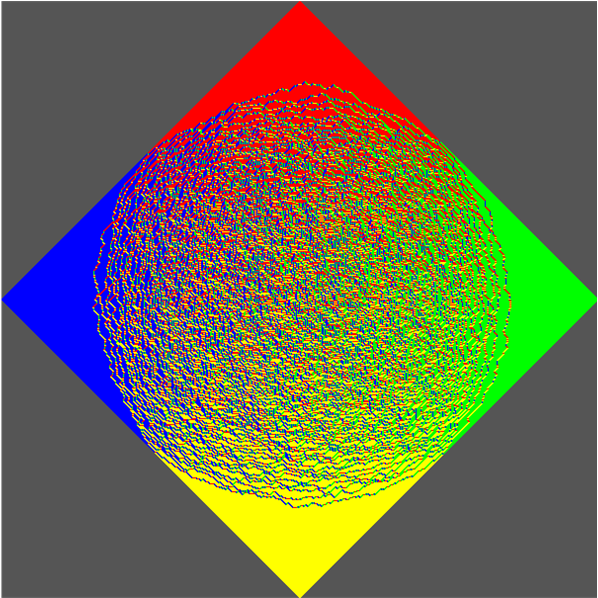
\includegraphics[scale=0.5]{aztecdiamond.png}
\centering
\end{figure}
\end{frame}

\begin{frame}{Table of contents}
\tableofcontents
\end{frame}





 
 
\begin{frame}{Mathematical Aspect}
\section{Mathematical Aspect}
\framesubtitle{Plan}
 \begin{itemize}
  \vspace*{\stretch{1}}
  \item  Aztec Diamond
     \item Random Tiling
     \item Theorem
  \vspace*{\stretch{1}}   
 \end{itemize}

 \end{frame}
 
 
   \begin{frame}{Mathematical Aspect}
\framesubtitle{Aztec Diamond}
\begin{itemize}
\begin{center}
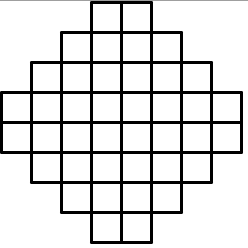
\includegraphics[scale=0.55]{Graph1.png}
\end{center}
\end{itemize}

\begin{itemize}
\begin{itemize}
  \item Combinatorial Mathematics \\
     \item Property : square lattice whose centers (x,y) satisfy $|x| + |y| \leq n$
     
     
 \end{itemize}
\end{itemize}
\end{frame}
 
 
 \begin{frame}{Mathematical Aspect}
 \framesubtitle{Random tiling}
 \begin{itemize}
    \begin{center}
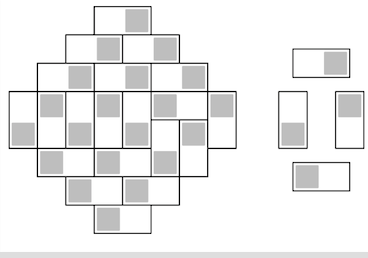
\includegraphics[scale=0.55]{Echec.png}

\end{center}
 \end{itemize}
 \begin{itemize}
     \item Checker
     \item Horizontal - Vertical
     
     
 \end{itemize}
 \end{frame}
  
 \begin{frame}{Mathematical Aspect}
 \framesubtitle{Random tiling}
 \begin{itemize}
    \begin{center}
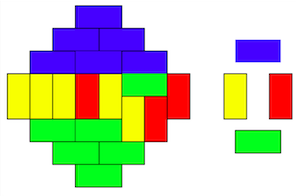
\includegraphics[scale=0.55]{Echec2.png}
\end{center}
 \end{itemize}
 \begin{itemize}
     \item Four different cases
      
     
 \end{itemize}

 
 \end{frame}
 
 \begin{frame}{Mathematical Aspect}
 \framesubtitle{Random tiling}
 \begin{itemize}
    \begin{center}
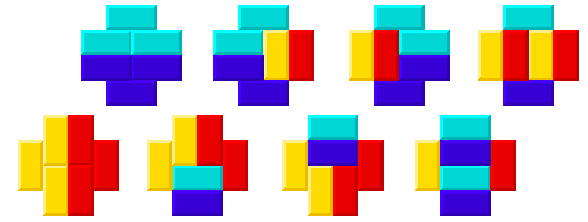
\includegraphics[scale=0.45]{Ti1.png}
\end{center}
 \end{itemize}
 \begin{itemize}
     \item 8 random tilings
      \item Aztec Diamond $n = 2$
        \item Random tillings : $2^{n(n+1)/2}$
     
 \end{itemize}

 
 \end{frame}
 
 \begin{frame}{Mathematical Aspect}
 \framesubtitle{Theorem}
 \begin{itemize}
    \begin{center}
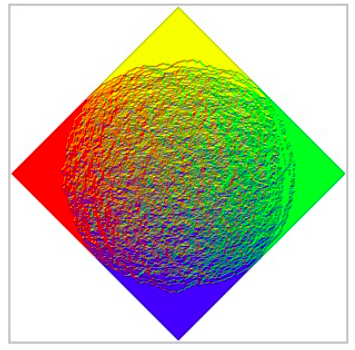
\includegraphics[scale=0.45]{A1.png}
\end{center}
 \end{itemize}
 \begin{itemize}
      \item Aztec Diamond $n = 300$
       
     
 \end{itemize}

 
 \end{frame}
 
 
\begin{frame}{Mathematical Aspect}
 \framesubtitle{Theorem}

\textbf{Theorem : ( Jockush, J.Propp and P.Shor, 1995)}\\

For all  $\epsilon > 0 $ , with probability tending to 1, outside the magnified inscribed circle $(1 + \epsilon)$ time, all dominoes are oriented in deterministic ways :
- Vertical in the right and left corners
- Horizontal up and down
\vspace{0.5cm}
\begin{itemize}
      \item Sen-Peng Eu Tung-Shan 
        \item Tilings and Schroeder's moth
       
     
 \end{itemize}
   
 \end{frame}
 



























 \begin{frame}{Numerical Aspect}
 \frametitle{Numerical Aspect}
 \section{Numerical Aspect}


 \begin{itemize}
 \vspace*{\stretch{1}}
 
  \item I - Domino class
     \item II - AztecDiamond Class
     \item III - Main
     
 \vspace*{\stretch{1}}     
 \end{itemize}

 \end{frame}






\begin{frame}{Numerical Aspect}
 \framesubtitle{Domino class}

\begin{itemize}
\vspace*{\stretch{1}}
    \item  What does the Domino class do?
    \item usefull packages : numpy, pygame
    \item $\_ init \_$ 
    \item $gen\_rect$
    \item $step$
\vspace*{\stretch{1}}
\end{itemize} 


\end{frame}







\begin{frame}{Numerical Aspect}
 \framesubtitle{AztecDiamond class}

\begin{itemize}
    \item What does the AztecDiamond class do?
    \item usefull packages and class : numpy, pygame, random, Domino class \
    \item 14 functions:
    \item  $\_$init$\_$
    \item generate$\_$diamond$\_$array
    \item production$\_$rect$\_$grille
    \item etape$\_$pavage: uses 5 other functions
    \item draw : uses 5 other functions
\end{itemize} 


\end{frame}



\begin{frame}{Numerical Aspect}
 \framesubtitle{draw function}

\begin{itemize}
\vspace*{\stretch{1}}
    \item  gerer$\_$evenements 
    \item ecran$\_$vide 
    \item dessin$\_$grille 
    \item dessin$\_$tuiles 
    \item dessin$\_$commentaire 
\vspace*{\stretch{1}}    
\end{itemize} 


\end{frame}




\begin{frame}{Numerical Aspect}
 \framesubtitle{etape$\_$pavage function}

\begin{itemize}
\vspace*{\stretch{1}}
    \item draw 
    \item  augmentation$\_$taille 
    \item suppression$\_$oppose 
    \item move$\_$tiles 
    \item remplissage$\_$deuxdeux 
\vspace*{\stretch{1}}    
\end{itemize} 


\end{frame}






\begin{frame}{Numerical Aspect}
 \framesubtitle{main function}

\begin{itemize}
    \item Is the execution point  of our program
    \item diamond = AztecDiamond(order=1)
    \item diamond.remplissage$_$deuxdeux()
    \item diamond.etape$_$pavage(draw=True)
    
    \begin{figure}[t]
\includegraphics[width=4cm]{aztec_order1.png}
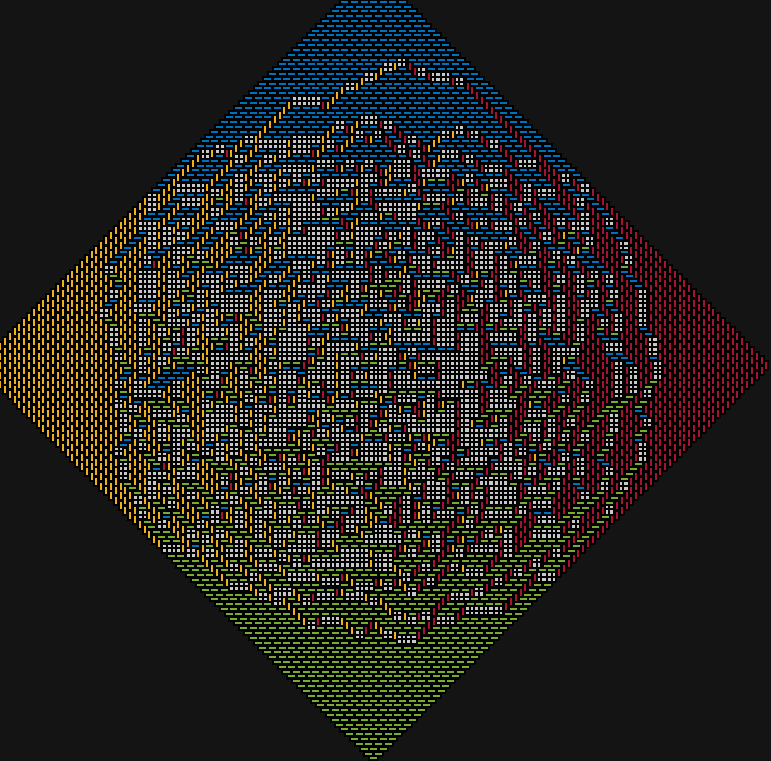
\includegraphics[width=4cm]{aztec_order70.png}

\centering
\end{figure}

\end{itemize} 


\end{frame}

















\begin{frame}
\frametitle{Pytest}
\section{Pytest}

\setbeamertemplate{blocks}[rounded][shadow=false] 
\begin{rows}
  \begin{row}
  \begin{block}{Class Domino}
 Test the domino with the order 5, the localisation (3,2) and the position west O 
  
\begin{figure}[!h]
    \begin{center}
   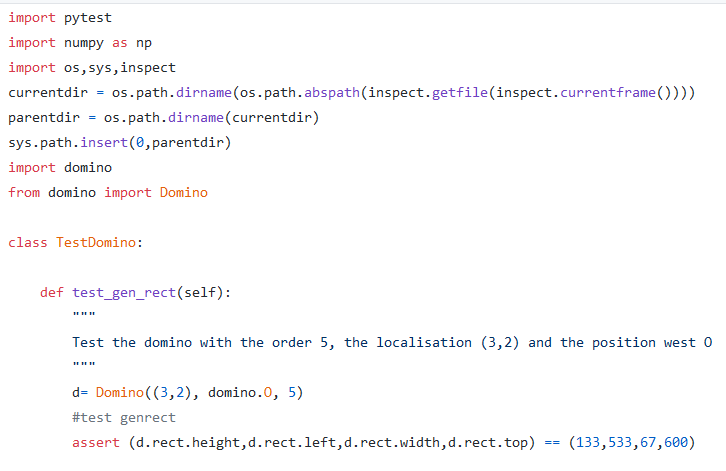
\includegraphics[width=6cm]{pytestdomino.png}
   \end{center}
    \end{figure}
  \end{block}   
  \end{row}
 \end{rows}

\end{frame}

\begin{frame}
\frametitle{Pytest}
\setbeamertemplate{blocks}[rounded][shadow=false] 
\begin{rows}
  \begin{row}
  \begin{block}{Class Aztecdiamond}
 This function test if the diamond of the aztec diamond in order 5 equals with what we expected.
  
\begin{figure}[!h]
    \begin{center}
   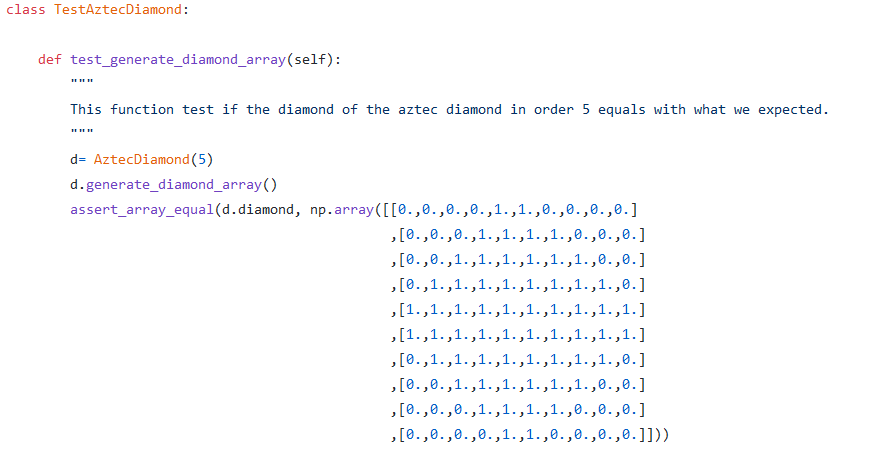
\includegraphics[width=6cm]{pytestaztec.png}
   \end{center}
    \end{figure}
  \end{block}   
  \end{row}
 \end{rows}

\end{frame}


\begin{frame}

\frametitle{Install}

\begin{itemize}
    \item First, you have to check that all python packages in the requirements.txt file are installed in the correct version. To make sure if every dependencies are installed in the right version you can simply run in a prompt:
    \begin{figure}[!h]
    \begin{center}
   
\includegraphics[width=6cm]{pipinstall.png}
   \end{center}
    \end{figure}
    \item In order to put the package for Aztec Diamonds, you have to run in its command prompt the following line.
    \begin{figure}[!h]
    \begin{center}
   
\includegraphics[width=10cm]{pipinstall2.png}
   \end{center}
    \end{figure}
    \item We recommend to clone the entire folder and them install it (git must be functional on your computer)
    \begin{figure}[!h]
    \begin{center}
   
\includegraphics[width=10cm]{pipinstall3.png}
   \end{center}
    \end{figure}
\end{itemize}
\end{frame}

\begin{frame}{Git and Doc}
\section{Git and Doc}
\begin{itemize}
    \item Content of the git : Beamer , file src , test ...
    \item Content of the doc ( module sphinx) : mathematical aspects, code details, resources and contacts.
\begin{center}
    
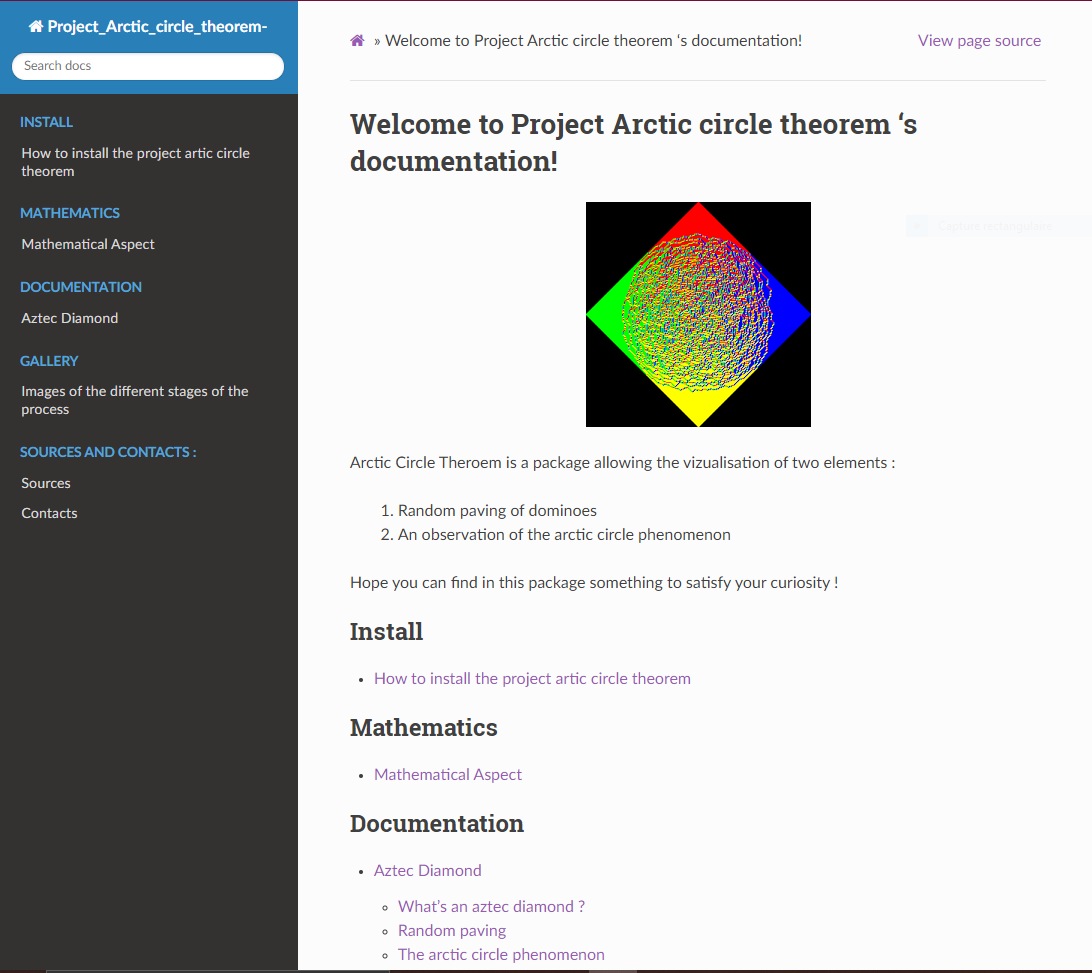
\includegraphics[width=6cm]{paged'acceuil.PNG}    
\end{center}
\end{itemize}
\end{frame}


\begin{frame}
\frametitle{Conclusion}
\begin{center}
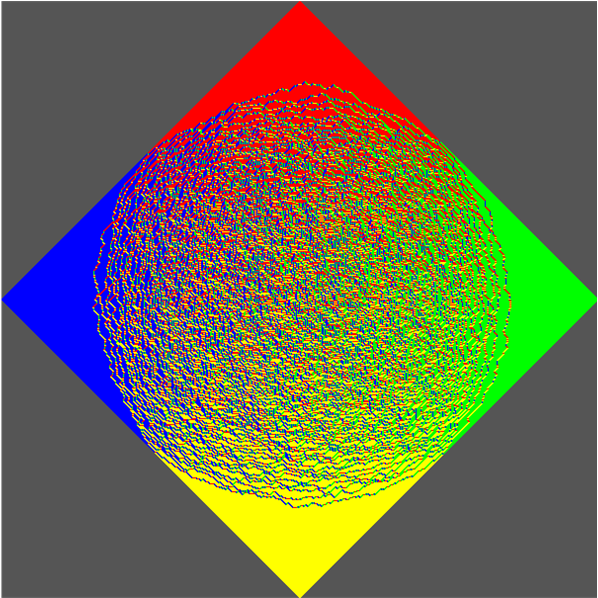
\includegraphics[scale=0.15]{aztecdiamond.png}
\end{center}

\begin{itemize}
\item general conclusion 
\item Limit of our packages

\item Teamwork
\begin{figure}[b]
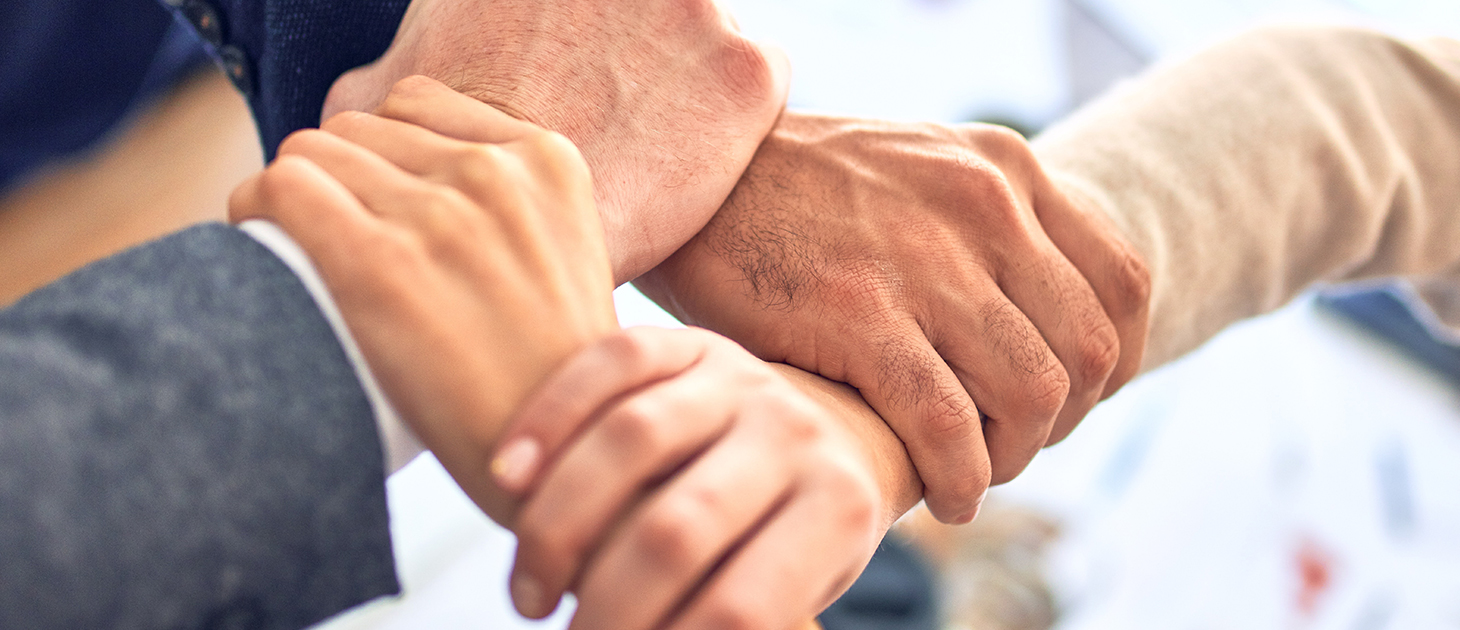
\includegraphics[width=8cm]{hands-team-work.jpg}
\centering
\end{figure}
\end{itemize}
\end{frame}


\end{document}







































